% visnet_arch_schematic.tex
% Compile: pdflatex visnet_arch_schematic.tex
\documentclass[border=8pt,tikz]{standalone}
\usepackage{tikz}
\usetikzlibrary{positioning,arrows.meta,fit,backgrounds,calc}

\begin{document}
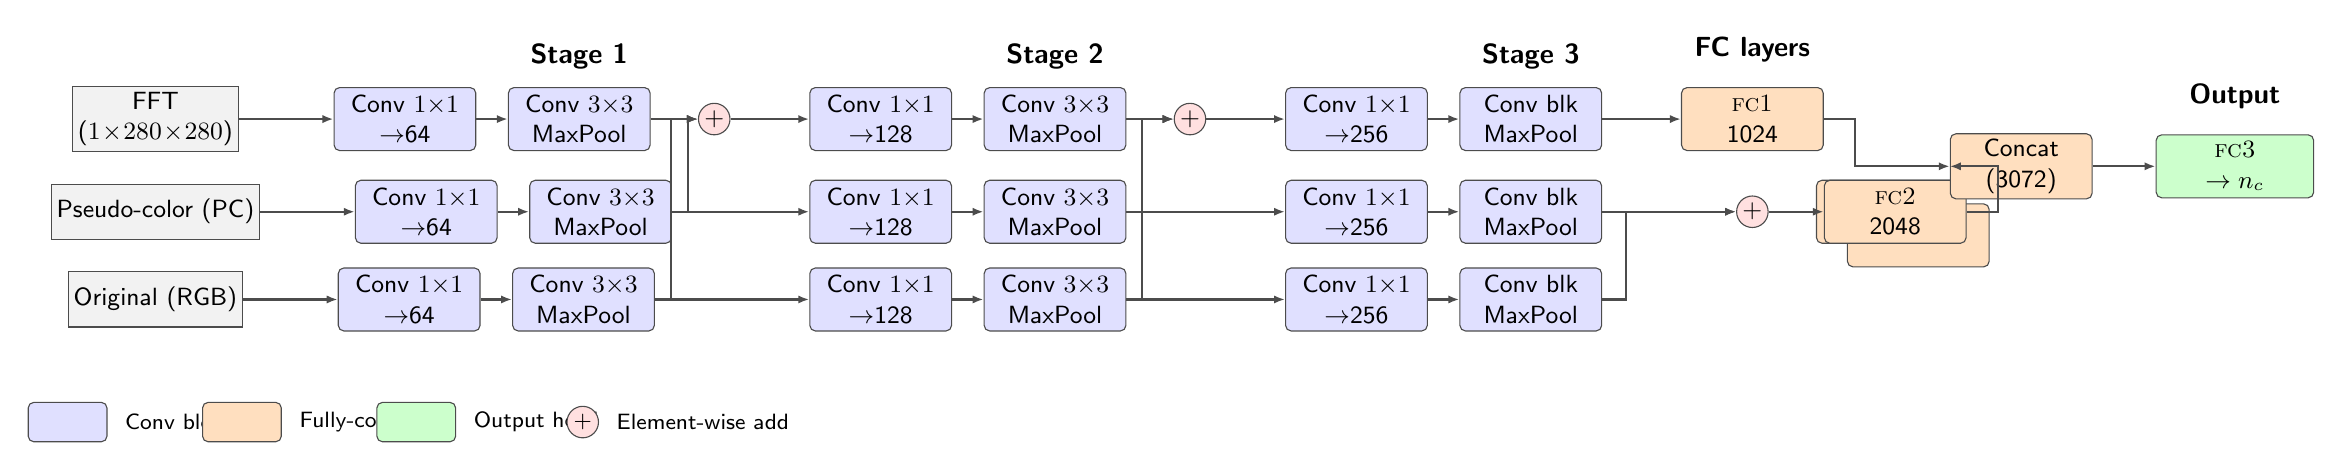
\begin{tikzpicture}[
  font=\sffamily\small,
  every node/.style={align=center},
  conv/.style ={rectangle, rounded corners=2pt, draw=black!70, fill=blue!12,
                minimum width=18mm, minimum height=8mm, inner sep=2pt},
  fc/.style   ={rectangle, rounded corners=2pt, draw=black!70, fill=orange!25,
                minimum width=18mm, minimum height=8mm, inner sep=2pt},
  head/.style ={rectangle, rounded corners=2pt, draw=black!70, fill=green!20,
                minimum width=20mm, minimum height=8mm, inner sep=2pt},
  inp/.style  ={rectangle, draw=black!70, fill=gray!10,
                minimum width=18mm, minimum height=7mm, inner sep=2pt},
  sum/.style  ={circle, draw=black!70, fill=red!12, inner sep=0pt, minimum size=4mm},
  arrow/.style={-{Latex[length=1.4mm]}, thick, draw=black!70},
  dash/.style ={dashed, draw=black!50, thick},
]

% -------- inputs ----------------------------------------------------------
\node[inp] (in1) {FFT\\($1\!\times\!280\!\times\!280$)};
\node[inp, below=4mm of in1] (in2) {Pseudo-color (PC)};
\node[inp, below=4mm of in2] (in3) {Original (RGB)};

% -------- Stage 1 ---------------------------------------------------------
\node[conv, right=12mm of in1] (s1a) {Conv $1{\times}1$\\$\to$64};
\node[conv, right=12mm of in2] (s2a) {Conv $1{\times}1$\\$\to$64};
\node[conv, right=12mm of in3] (s3a) {Conv $1{\times}1$\\$\to$64};

\node[conv, right=4mm of s1a] (s1b) {Conv $3{\times}3$\\MaxPool};
\node[conv, right=4mm of s2a] (s2b) {Conv $3{\times}3$\\MaxPool};
\node[conv, right=4mm of s3a] (s3b) {Conv $3{\times}3$\\MaxPool};

% Fusion 1 (after stage 1): s1 += s2 + s3
\node[sum, right=6mm of s1b] (sum1) {$+$};

% -------- Stage 2 ---------------------------------------------------------
\node[conv, right=10mm of sum1] (s1c) {Conv $1{\times}1$\\$\to$128};
\node[conv] (s2c) at (s1c |- s2b) {Conv $1{\times}1$\\$\to$128};
\node[conv] (s3c) at (s1c |- s3b) {Conv $1{\times}1$\\$\to$128};

\node[conv, right=4mm of s1c] (s1d) {Conv $3{\times}3$\\MaxPool};
\node[conv, right=4mm of s2c] (s2d) {Conv $3{\times}3$\\MaxPool};
\node[conv, right=4mm of s3c] (s3d) {Conv $3{\times}3$\\MaxPool};

\node[sum, right=6mm of s1d] (sum2) {$+$};

% -------- Stage 3 ---------------------------------------------------------
\node[conv, right=10mm of sum2] (s1e) {Conv $1{\times}1$\\$\to$256};
\node[conv] (s2e) at (s1e |- s2d) {Conv $1{\times}1$\\$\to$256};
\node[conv] (s3e) at (s1e |- s3d) {Conv $1{\times}1$\\$\to$256};

\node[conv, right=4mm of s1e] (s1f) {Conv blk\\MaxPool};
\node[conv, right=4mm of s2e] (s2f) {Conv blk\\MaxPool};
\node[conv, right=4mm of s3e] (s3f) {Conv blk\\MaxPool};

% -------- FC --------------------------------------------------------------
\node[fc, right=10mm of s1f] (fc1) {\textsc{fc1}\\1024};
\node[sum] (sum3) at (s2f.east -| fc1.center) {$+$};
\node[fc, right=6mm of sum3] (fc2) {\textsc{fc2}\\2048};

% Move fc2 down to be at midpoint between s2,s3
\node[fc] (fc2X) at ($(s2f.east -| fc1.east) + (12mm,-3mm)$) {};
% Simpler: place fc2 explicitly
\node[fc] at (sum3) [right=8mm of sum3,xshift=-1mm] (fc2real) {\textsc{fc2}\\2048};

% concat & fc3
\node[fc, right=16mm of fc1, yshift=-6mm] (concat) {Concat\\(3072)};
\node[head, right=8mm of concat] (fc3) {\textsc{fc3}\\$\to n_c$};

% -------- arrows ----------------------------------------------------------
\foreach \a/\b in {in1/s1a, in2/s2a, in3/s3a,
                   s1a/s1b, s2a/s2b, s3a/s3b}
  \draw[arrow] (\a) -- (\b);

% stage1 fusion
\draw[arrow] (s1b) -- (sum1);
\draw[arrow] (s2b.east) -- ++(2mm,0) |- (sum1);
\draw[arrow] (s3b.east) -- ++(2mm,0) |- (sum1);

\draw[arrow] (sum1) -- (s1c);
\draw[arrow] (s2b) -- (s2c);
\draw[arrow] (s3b) -- (s3c);

\foreach \a/\b in {s1c/s1d, s2c/s2d, s3c/s3d}
  \draw[arrow] (\a) -- (\b);

% stage2 fusion
\draw[arrow] (s1d) -- (sum2);
\draw[arrow] (s2d.east) -- ++(2mm,0) |- (sum2);
\draw[arrow] (s3d.east) -- ++(2mm,0) |- (sum2);

\draw[arrow] (sum2) -- (s1e);
\draw[arrow] (s2d) -- (s2e);
\draw[arrow] (s3d) -- (s3e);

\foreach \a/\b in {s1e/s1f, s2e/s2f, s3e/s3f}
  \draw[arrow] (\a) -- (\b);

% to fc
\draw[arrow] (s1f) -- (fc1);
\draw[arrow] (s2f.east) -- ++(3mm,0) |- (sum3);
\draw[arrow] (s3f.east) -- ++(3mm,0) |- (sum3);
\draw[arrow] (sum3) -- (fc2real);

% concat
\draw[arrow] (fc1.east) -- ++(4mm,0) |- (concat.west);
\draw[arrow] (fc2real.east) -- ++(4mm,0) |- (concat.west);
\draw[arrow] (concat) -- (fc3);

% -------- stage labels ----------------------------------------------------
\node[above=1mm of s1b, font=\sffamily\bfseries] {Stage 1};
\node[above=1mm of s1d, font=\sffamily\bfseries] {Stage 2};
\node[above=1mm of s1f, font=\sffamily\bfseries] {Stage 3};
\node[above=2mm of fc1, font=\sffamily\bfseries] {FC layers};
\node[above=2mm of fc3, font=\sffamily\bfseries] {Output};

% -------- legend ----------------------------------------------------------
\begin{scope}[shift={($(in3.south west)+(0,-12mm)$)}, font=\sffamily\footnotesize]
  \node[conv, minimum width=10mm, minimum height=5mm] (lg1) {};
  \node[right=1mm of lg1] {Conv block};
  \node[fc,   minimum width=10mm, minimum height=5mm, right=12mm of lg1] (lg2) {};
  \node[right=1mm of lg2] {Fully-connected};
  \node[head, minimum width=10mm, minimum height=5mm, right=12mm of lg2] (lg3) {};
  \node[right=1mm of lg3] {Output head};
  \node[sum, right=14mm of lg3] (lg4) {$+$};
  \node[right=1mm of lg4] {Element-wise add};
\end{scope}

\end{tikzpicture}
\end{document}